\chapter*{Proposition 40}



\begin{figure*}[ht]
    \begin{center}
    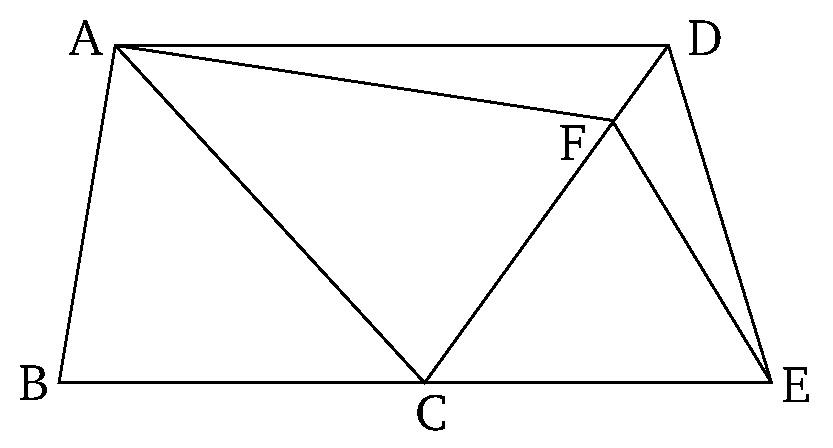
\includegraphics[width=0.5\linewidth]{figures/fig40e.eps}
    \label{fig:prop_40}
    \end{center}
\end{figure*}

Equal triangles which are on equal bases, and on the same side, are also
between the same parallels.

Let $ABC$ and $CDE$ be equal triangles on the equal bases $BC$ and $CE$ (respectively), and on the same side (of $BE$). I say that they are also between
the same parallels.

For let $AD$ have been joined. I say that $AD$ is parallel to $BE$.

For if not, let $AF$ have been drawn through $A$ parallel to $BE$ [Prop.~1.31],
and let $FE$ have been joined. Thus, triangle $ABC$ is equal to triangle
$FCE$. For they are on equal bases, $BC$ and $CE$, and between the same
parallels, $BE$ and $AF$ [Prop.~1.38]. But, triangle $ABC$ is equal to [triangle] $DCE$.
Thus, [triangle] $DCE$ is also equal to triangle $FCE$, the greater to the
lesser. The very thing is impossible. 
Thus, $AF$ is not parallel to $BE$. Similarly, we can show that neither (is)
any other (straight-line) than $AD$. Thus, $AD$ is parallel to $BE$.

Thus, equal triangles which are on equal bases, and on the same side, are also
between the same parallels. (Which is) the very thing it was required to show.


\section*{Commentary}

\begin{proposition}\label{proposition_40}\lean{Elements.Book1.proposition_40}\leanok
    If
\end{proposition}
\begin{proof}
    \uses{proposition_31,proposition_38}\leanok
\end{proof}
